% !TEX encoding = UTF-8 Unicode
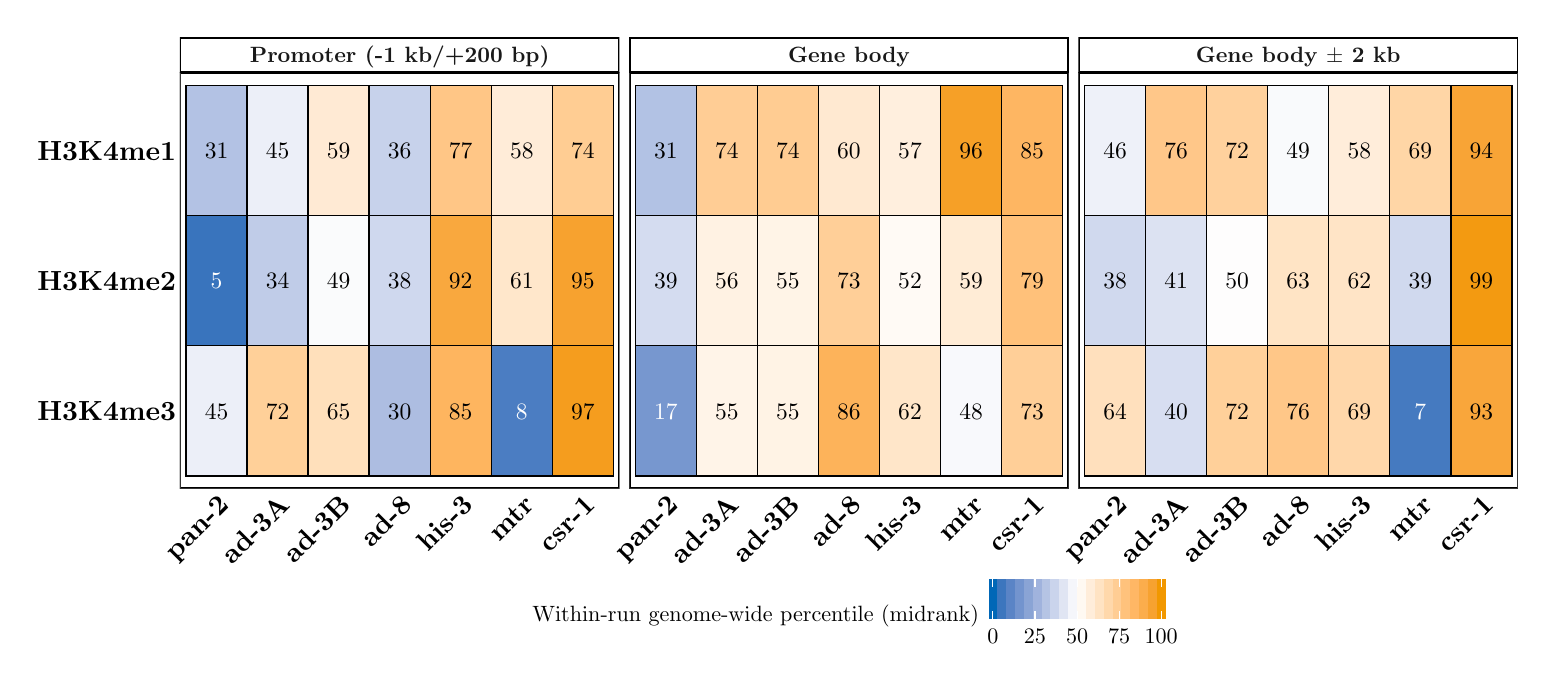
\begin{tikzpicture}[x=1pt,y=1pt]
\definecolor{fillColor}{RGB}{255,255,255}
\path[use as bounding box,fill=fillColor,fill opacity=0.00] (0,0) rectangle (542.02,231.26);
\begin{scope}
\path[clip] (  0.00,  0.00) rectangle (542.02,231.26);
\definecolor{drawColor}{RGB}{255,255,255}
\definecolor{fillColor}{RGB}{255,255,255}

\path[draw=drawColor,line width= 0.7pt,line join=round,line cap=round,fill=fillColor] ( -0.00,  0.00) rectangle (542.02,231.26);
\end{scope}
\begin{scope}
\path[clip] ( 55.01, 64.56) rectangle (213.85,215.09);
\definecolor{drawColor}{RGB}{0,0,0}
\definecolor{fillColor}{RGB}{255,255,255}

\path[draw=drawColor,line width= 1.1pt,line join=round,line cap=round,fill=fillColor] ( 55.01, 64.56) rectangle (213.85,215.09);
\definecolor{fillColor}{RGB}{179,194,228}

\path[draw=drawColor,line width= 0.5pt,fill=fillColor] ( 57.21,163.34) rectangle ( 79.27,210.38);
\definecolor{fillColor}{RGB}{236,239,248}

\path[draw=drawColor,line width= 0.5pt,fill=fillColor] ( 79.27,163.34) rectangle (101.33,210.38);
\definecolor{fillColor}{RGB}{255,234,212}

\path[draw=drawColor,line width= 0.5pt,fill=fillColor] (101.33,163.34) rectangle (123.40,210.38);
\definecolor{fillColor}{RGB}{199,210,235}

\path[draw=drawColor,line width= 0.5pt,fill=fillColor] (123.40,163.34) rectangle (145.46,210.38);
\definecolor{fillColor}{RGB}{255,198,134}

\path[draw=drawColor,line width= 0.5pt,fill=fillColor] (145.46,163.34) rectangle (167.52,210.38);
\definecolor{fillColor}{RGB}{255,236,216}

\path[draw=drawColor,line width= 0.5pt,fill=fillColor] (167.52,163.34) rectangle (189.58,210.38);
\definecolor{fillColor}{RGB}{255,205,147}

\path[draw=drawColor,line width= 0.5pt,fill=fillColor] (189.58,163.34) rectangle (211.64,210.38);
\definecolor{fillColor}{RGB}{57,116,189}

\path[draw=drawColor,line width= 0.5pt,fill=fillColor] ( 57.21,116.31) rectangle ( 79.27,163.34);
\definecolor{fillColor}{RGB}{192,204,232}

\path[draw=drawColor,line width= 0.5pt,fill=fillColor] ( 79.27,116.31) rectangle (101.33,163.34);
\definecolor{fillColor}{RGB}{250,251,252}

\path[draw=drawColor,line width= 0.5pt,fill=fillColor] (101.33,116.31) rectangle (123.40,163.34);
\definecolor{fillColor}{RGB}{207,216,238}

\path[draw=drawColor,line width= 0.5pt,fill=fillColor] (123.40,116.31) rectangle (145.46,163.34);
\definecolor{fillColor}{RGB}{249,168,62}

\path[draw=drawColor,line width= 0.5pt,fill=fillColor] (145.46,116.31) rectangle (167.52,163.34);
\definecolor{fillColor}{RGB}{255,231,203}

\path[draw=drawColor,line width= 0.5pt,fill=fillColor] (167.52,116.31) rectangle (189.58,163.34);
\definecolor{fillColor}{RGB}{247,162,47}

\path[draw=drawColor,line width= 0.5pt,fill=fillColor] (189.58,116.31) rectangle (211.64,163.34);
\definecolor{fillColor}{RGB}{236,239,248}

\path[draw=drawColor,line width= 0.5pt,fill=fillColor] ( 57.21, 69.27) rectangle ( 79.27,116.31);
\definecolor{fillColor}{RGB}{255,208,153}

\path[draw=drawColor,line width= 0.5pt,fill=fillColor] ( 79.27, 69.27) rectangle (101.33,116.31);
\definecolor{fillColor}{RGB}{255,224,187}

\path[draw=drawColor,line width= 0.5pt,fill=fillColor] (101.33, 69.27) rectangle (123.40,116.31);
\definecolor{fillColor}{RGB}{173,189,225}

\path[draw=drawColor,line width= 0.5pt,fill=fillColor] (123.40, 69.27) rectangle (145.46,116.31);
\definecolor{fillColor}{RGB}{254,181,95}

\path[draw=drawColor,line width= 0.5pt,fill=fillColor] (145.46, 69.27) rectangle (167.52,116.31);
\definecolor{fillColor}{RGB}{75,125,194}

\path[draw=drawColor,line width= 0.5pt,fill=fillColor] (167.52, 69.27) rectangle (189.58,116.31);
\definecolor{fillColor}{RGB}{245,157,30}

\path[draw=drawColor,line width= 0.5pt,fill=fillColor] (189.58, 69.27) rectangle (211.64,116.31);

\node[text=drawColor,anchor=base,inner sep=0pt, outer sep=0pt, scale=  0.85] at ( 68.24,183.93) {31};

\node[text=drawColor,anchor=base,inner sep=0pt, outer sep=0pt, scale=  0.85] at ( 90.30,183.93) {45};

\node[text=drawColor,anchor=base,inner sep=0pt, outer sep=0pt, scale=  0.85] at (112.36,183.93) {59};

\node[text=drawColor,anchor=base,inner sep=0pt, outer sep=0pt, scale=  0.85] at (134.43,183.93) {36};

\node[text=drawColor,anchor=base,inner sep=0pt, outer sep=0pt, scale=  0.85] at (156.49,183.93) {77};

\node[text=drawColor,anchor=base,inner sep=0pt, outer sep=0pt, scale=  0.85] at (178.55,183.93) {58};

\node[text=drawColor,anchor=base,inner sep=0pt, outer sep=0pt, scale=  0.85] at (200.61,183.93) {74};
\definecolor{drawColor}{RGB}{255,255,255}

\node[text=drawColor,anchor=base,inner sep=0pt, outer sep=0pt, scale=  0.85] at ( 68.24,136.89) {5};
\definecolor{drawColor}{RGB}{0,0,0}

\node[text=drawColor,anchor=base,inner sep=0pt, outer sep=0pt, scale=  0.85] at ( 90.30,136.89) {34};

\node[text=drawColor,anchor=base,inner sep=0pt, outer sep=0pt, scale=  0.85] at (112.36,136.89) {49};

\node[text=drawColor,anchor=base,inner sep=0pt, outer sep=0pt, scale=  0.85] at (134.43,136.89) {38};

\node[text=drawColor,anchor=base,inner sep=0pt, outer sep=0pt, scale=  0.85] at (156.49,136.89) {92};

\node[text=drawColor,anchor=base,inner sep=0pt, outer sep=0pt, scale=  0.85] at (178.55,136.89) {61};

\node[text=drawColor,anchor=base,inner sep=0pt, outer sep=0pt, scale=  0.85] at (200.61,136.89) {95};

\node[text=drawColor,anchor=base,inner sep=0pt, outer sep=0pt, scale=  0.85] at ( 68.24, 89.85) {45};

\node[text=drawColor,anchor=base,inner sep=0pt, outer sep=0pt, scale=  0.85] at ( 90.30, 89.85) {72};

\node[text=drawColor,anchor=base,inner sep=0pt, outer sep=0pt, scale=  0.85] at (112.36, 89.85) {65};

\node[text=drawColor,anchor=base,inner sep=0pt, outer sep=0pt, scale=  0.85] at (134.43, 89.85) {30};

\node[text=drawColor,anchor=base,inner sep=0pt, outer sep=0pt, scale=  0.85] at (156.49, 89.85) {85};
\definecolor{drawColor}{RGB}{255,255,255}

\node[text=drawColor,anchor=base,inner sep=0pt, outer sep=0pt, scale=  0.85] at (178.55, 89.85) {8};
\definecolor{drawColor}{RGB}{0,0,0}

\node[text=drawColor,anchor=base,inner sep=0pt, outer sep=0pt, scale=  0.85] at (200.61, 89.85) {97};
\definecolor{drawColor}{gray}{0.20}

\path[draw=drawColor,line width= 0.7pt,line join=round,line cap=round] ( 55.01, 64.56) rectangle (213.85,215.09);
\end{scope}
\begin{scope}
\path[clip] (217.35, 64.56) rectangle (376.19,215.09);
\definecolor{drawColor}{RGB}{0,0,0}
\definecolor{fillColor}{RGB}{255,255,255}

\path[draw=drawColor,line width= 1.1pt,line join=round,line cap=round,fill=fillColor] (217.35, 64.56) rectangle (376.19,215.09);
\definecolor{fillColor}{RGB}{178,194,228}

\path[draw=drawColor,line width= 0.5pt,fill=fillColor] (219.55,163.34) rectangle (241.61,210.38);
\definecolor{fillColor}{RGB}{255,205,149}

\path[draw=drawColor,line width= 0.5pt,fill=fillColor] (241.61,163.34) rectangle (263.67,210.38);
\definecolor{fillColor}{RGB}{255,204,146}

\path[draw=drawColor,line width= 0.5pt,fill=fillColor] (263.67,163.34) rectangle (285.73,210.38);
\definecolor{fillColor}{RGB}{255,233,209}

\path[draw=drawColor,line width= 0.5pt,fill=fillColor] (285.73,163.34) rectangle (307.80,210.38);
\definecolor{fillColor}{RGB}{255,239,222}

\path[draw=drawColor,line width= 0.5pt,fill=fillColor] (307.80,163.34) rectangle (329.86,210.38);
\definecolor{fillColor}{RGB}{246,160,39}

\path[draw=drawColor,line width= 0.5pt,fill=fillColor] (329.86,163.34) rectangle (351.92,210.38);
\definecolor{fillColor}{RGB}{254,182,98}

\path[draw=drawColor,line width= 0.5pt,fill=fillColor] (351.92,163.34) rectangle (373.98,210.38);
\definecolor{fillColor}{RGB}{212,220,240}

\path[draw=drawColor,line width= 0.5pt,fill=fillColor] (219.55,116.31) rectangle (241.61,163.34);
\definecolor{fillColor}{RGB}{255,242,227}

\path[draw=drawColor,line width= 0.5pt,fill=fillColor] (241.61,116.31) rectangle (263.67,163.34);
\definecolor{fillColor}{RGB}{255,244,231}

\path[draw=drawColor,line width= 0.5pt,fill=fillColor] (263.67,116.31) rectangle (285.73,163.34);
\definecolor{fillColor}{RGB}{255,207,152}

\path[draw=drawColor,line width= 0.5pt,fill=fillColor] (285.73,116.31) rectangle (307.80,163.34);
\definecolor{fillColor}{RGB}{255,250,245}

\path[draw=drawColor,line width= 0.5pt,fill=fillColor] (307.80,116.31) rectangle (329.86,163.34);
\definecolor{fillColor}{RGB}{255,236,214}

\path[draw=drawColor,line width= 0.5pt,fill=fillColor] (329.86,116.31) rectangle (351.92,163.34);
\definecolor{fillColor}{RGB}{255,193,122}

\path[draw=drawColor,line width= 0.5pt,fill=fillColor] (351.92,116.31) rectangle (373.98,163.34);
\definecolor{fillColor}{RGB}{119,151,207}

\path[draw=drawColor,line width= 0.5pt,fill=fillColor] (219.55, 69.27) rectangle (241.61,116.31);
\definecolor{fillColor}{RGB}{255,244,232}

\path[draw=drawColor,line width= 0.5pt,fill=fillColor] (241.61, 69.27) rectangle (263.67,116.31);
\definecolor{fillColor}{RGB}{255,243,229}

\path[draw=drawColor,line width= 0.5pt,fill=fillColor] (263.67, 69.27) rectangle (285.73,116.31);
\definecolor{fillColor}{RGB}{253,179,90}

\path[draw=drawColor,line width= 0.5pt,fill=fillColor] (285.73, 69.27) rectangle (307.80,116.31);
\definecolor{fillColor}{RGB}{255,230,201}

\path[draw=drawColor,line width= 0.5pt,fill=fillColor] (307.80, 69.27) rectangle (329.86,116.31);
\definecolor{fillColor}{RGB}{248,249,252}

\path[draw=drawColor,line width= 0.5pt,fill=fillColor] (329.86, 69.27) rectangle (351.92,116.31);
\definecolor{fillColor}{RGB}{255,207,152}

\path[draw=drawColor,line width= 0.5pt,fill=fillColor] (351.92, 69.27) rectangle (373.98,116.31);

\node[text=drawColor,anchor=base,inner sep=0pt, outer sep=0pt, scale=  0.85] at (230.58,183.93) {31};

\node[text=drawColor,anchor=base,inner sep=0pt, outer sep=0pt, scale=  0.85] at (252.64,183.93) {74};

\node[text=drawColor,anchor=base,inner sep=0pt, outer sep=0pt, scale=  0.85] at (274.70,183.93) {74};

\node[text=drawColor,anchor=base,inner sep=0pt, outer sep=0pt, scale=  0.85] at (296.77,183.93) {60};

\node[text=drawColor,anchor=base,inner sep=0pt, outer sep=0pt, scale=  0.85] at (318.83,183.93) {57};

\node[text=drawColor,anchor=base,inner sep=0pt, outer sep=0pt, scale=  0.85] at (340.89,183.93) {96};

\node[text=drawColor,anchor=base,inner sep=0pt, outer sep=0pt, scale=  0.85] at (362.95,183.93) {85};

\node[text=drawColor,anchor=base,inner sep=0pt, outer sep=0pt, scale=  0.85] at (230.58,136.89) {39};

\node[text=drawColor,anchor=base,inner sep=0pt, outer sep=0pt, scale=  0.85] at (252.64,136.89) {56};

\node[text=drawColor,anchor=base,inner sep=0pt, outer sep=0pt, scale=  0.85] at (274.70,136.89) {55};

\node[text=drawColor,anchor=base,inner sep=0pt, outer sep=0pt, scale=  0.85] at (296.77,136.89) {73};

\node[text=drawColor,anchor=base,inner sep=0pt, outer sep=0pt, scale=  0.85] at (318.83,136.89) {52};

\node[text=drawColor,anchor=base,inner sep=0pt, outer sep=0pt, scale=  0.85] at (340.89,136.89) {59};

\node[text=drawColor,anchor=base,inner sep=0pt, outer sep=0pt, scale=  0.85] at (362.95,136.89) {79};
\definecolor{drawColor}{RGB}{255,255,255}

\node[text=drawColor,anchor=base,inner sep=0pt, outer sep=0pt, scale=  0.85] at (230.58, 89.85) {17};
\definecolor{drawColor}{RGB}{0,0,0}

\node[text=drawColor,anchor=base,inner sep=0pt, outer sep=0pt, scale=  0.85] at (252.64, 89.85) {55};

\node[text=drawColor,anchor=base,inner sep=0pt, outer sep=0pt, scale=  0.85] at (274.70, 89.85) {55};

\node[text=drawColor,anchor=base,inner sep=0pt, outer sep=0pt, scale=  0.85] at (296.77, 89.85) {86};

\node[text=drawColor,anchor=base,inner sep=0pt, outer sep=0pt, scale=  0.85] at (318.83, 89.85) {62};

\node[text=drawColor,anchor=base,inner sep=0pt, outer sep=0pt, scale=  0.85] at (340.89, 89.85) {48};

\node[text=drawColor,anchor=base,inner sep=0pt, outer sep=0pt, scale=  0.85] at (362.95, 89.85) {73};
\definecolor{drawColor}{gray}{0.20}

\path[draw=drawColor,line width= 0.7pt,line join=round,line cap=round] (217.35, 64.56) rectangle (376.19,215.09);
\end{scope}
\begin{scope}
\path[clip] (379.69, 64.56) rectangle (538.52,215.09);
\definecolor{drawColor}{RGB}{0,0,0}
\definecolor{fillColor}{RGB}{255,255,255}

\path[draw=drawColor,line width= 1.1pt,line join=round,line cap=round,fill=fillColor] (379.69, 64.56) rectangle (538.53,215.09);
\definecolor{fillColor}{RGB}{238,241,249}

\path[draw=drawColor,line width= 0.5pt,fill=fillColor] (381.89,163.34) rectangle (403.95,210.38);
\definecolor{fillColor}{RGB}{255,199,137}

\path[draw=drawColor,line width= 0.5pt,fill=fillColor] (403.95,163.34) rectangle (426.01,210.38);
\definecolor{fillColor}{RGB}{255,209,157}

\path[draw=drawColor,line width= 0.5pt,fill=fillColor] (426.01,163.34) rectangle (448.07,210.38);
\definecolor{fillColor}{RGB}{249,250,252}

\path[draw=drawColor,line width= 0.5pt,fill=fillColor] (448.07,163.34) rectangle (470.14,210.38);
\definecolor{fillColor}{RGB}{255,237,218}

\path[draw=drawColor,line width= 0.5pt,fill=fillColor] (470.14,163.34) rectangle (492.20,210.38);
\definecolor{fillColor}{RGB}{255,214,166}

\path[draw=drawColor,line width= 0.5pt,fill=fillColor] (492.20,163.34) rectangle (514.26,210.38);
\definecolor{fillColor}{RGB}{248,164,54}

\path[draw=drawColor,line width= 0.5pt,fill=fillColor] (514.26,163.34) rectangle (536.32,210.38);
\definecolor{fillColor}{RGB}{208,217,238}

\path[draw=drawColor,line width= 0.5pt,fill=fillColor] (381.89,116.31) rectangle (403.95,163.34);
\definecolor{fillColor}{RGB}{220,226,242}

\path[draw=drawColor,line width= 0.5pt,fill=fillColor] (403.95,116.31) rectangle (426.01,163.34);
\definecolor{fillColor}{RGB}{254,253,253}

\path[draw=drawColor,line width= 0.5pt,fill=fillColor] (426.01,116.31) rectangle (448.07,163.34);
\definecolor{fillColor}{RGB}{255,228,197}

\path[draw=drawColor,line width= 0.5pt,fill=fillColor] (448.07,116.31) rectangle (470.14,163.34);
\definecolor{fillColor}{RGB}{255,228,198}

\path[draw=drawColor,line width= 0.5pt,fill=fillColor] (470.14,116.31) rectangle (492.20,163.34);
\definecolor{fillColor}{RGB}{208,217,238}

\path[draw=drawColor,line width= 0.5pt,fill=fillColor] (492.20,116.31) rectangle (514.26,163.34);
\definecolor{fillColor}{RGB}{243,154,17}

\path[draw=drawColor,line width= 0.5pt,fill=fillColor] (514.26,116.31) rectangle (536.32,163.34);
\definecolor{fillColor}{RGB}{255,224,189}

\path[draw=drawColor,line width= 0.5pt,fill=fillColor] (381.89, 69.27) rectangle (403.95,116.31);
\definecolor{fillColor}{RGB}{215,222,241}

\path[draw=drawColor,line width= 0.5pt,fill=fillColor] (403.95, 69.27) rectangle (426.01,116.31);
\definecolor{fillColor}{RGB}{255,208,154}

\path[draw=drawColor,line width= 0.5pt,fill=fillColor] (426.01, 69.27) rectangle (448.07,116.31);
\definecolor{fillColor}{RGB}{255,199,136}

\path[draw=drawColor,line width= 0.5pt,fill=fillColor] (448.07, 69.27) rectangle (470.14,116.31);
\definecolor{fillColor}{RGB}{255,215,170}

\path[draw=drawColor,line width= 0.5pt,fill=fillColor] (470.14, 69.27) rectangle (492.20,116.31);
\definecolor{fillColor}{RGB}{69,122,192}

\path[draw=drawColor,line width= 0.5pt,fill=fillColor] (492.20, 69.27) rectangle (514.26,116.31);
\definecolor{fillColor}{RGB}{249,166,59}

\path[draw=drawColor,line width= 0.5pt,fill=fillColor] (514.26, 69.27) rectangle (536.32,116.31);

\node[text=drawColor,anchor=base,inner sep=0pt, outer sep=0pt, scale=  0.85] at (392.92,183.93) {46};

\node[text=drawColor,anchor=base,inner sep=0pt, outer sep=0pt, scale=  0.85] at (414.98,183.93) {76};

\node[text=drawColor,anchor=base,inner sep=0pt, outer sep=0pt, scale=  0.85] at (437.04,183.93) {72};

\node[text=drawColor,anchor=base,inner sep=0pt, outer sep=0pt, scale=  0.85] at (459.11,183.93) {49};

\node[text=drawColor,anchor=base,inner sep=0pt, outer sep=0pt, scale=  0.85] at (481.17,183.93) {58};

\node[text=drawColor,anchor=base,inner sep=0pt, outer sep=0pt, scale=  0.85] at (503.23,183.93) {69};

\node[text=drawColor,anchor=base,inner sep=0pt, outer sep=0pt, scale=  0.85] at (525.29,183.93) {94};

\node[text=drawColor,anchor=base,inner sep=0pt, outer sep=0pt, scale=  0.85] at (392.92,136.89) {38};

\node[text=drawColor,anchor=base,inner sep=0pt, outer sep=0pt, scale=  0.85] at (414.98,136.89) {41};

\node[text=drawColor,anchor=base,inner sep=0pt, outer sep=0pt, scale=  0.85] at (437.04,136.89) {50};

\node[text=drawColor,anchor=base,inner sep=0pt, outer sep=0pt, scale=  0.85] at (459.11,136.89) {63};

\node[text=drawColor,anchor=base,inner sep=0pt, outer sep=0pt, scale=  0.85] at (481.17,136.89) {62};

\node[text=drawColor,anchor=base,inner sep=0pt, outer sep=0pt, scale=  0.85] at (503.23,136.89) {39};

\node[text=drawColor,anchor=base,inner sep=0pt, outer sep=0pt, scale=  0.85] at (525.29,136.89) {99};

\node[text=drawColor,anchor=base,inner sep=0pt, outer sep=0pt, scale=  0.85] at (392.92, 89.85) {64};

\node[text=drawColor,anchor=base,inner sep=0pt, outer sep=0pt, scale=  0.85] at (414.98, 89.85) {40};

\node[text=drawColor,anchor=base,inner sep=0pt, outer sep=0pt, scale=  0.85] at (437.04, 89.85) {72};

\node[text=drawColor,anchor=base,inner sep=0pt, outer sep=0pt, scale=  0.85] at (459.11, 89.85) {76};

\node[text=drawColor,anchor=base,inner sep=0pt, outer sep=0pt, scale=  0.85] at (481.17, 89.85) {69};
\definecolor{drawColor}{RGB}{255,255,255}

\node[text=drawColor,anchor=base,inner sep=0pt, outer sep=0pt, scale=  0.85] at (503.23, 89.85) {7};
\definecolor{drawColor}{RGB}{0,0,0}

\node[text=drawColor,anchor=base,inner sep=0pt, outer sep=0pt, scale=  0.85] at (525.29, 89.85) {93};
\definecolor{drawColor}{gray}{0.20}

\path[draw=drawColor,line width= 0.7pt,line join=round,line cap=round] (379.69, 64.56) rectangle (538.53,215.09);
\end{scope}
\begin{scope}
\path[clip] ( 55.01,215.09) rectangle (213.85,227.76);
\definecolor{drawColor}{RGB}{0,0,0}
\definecolor{fillColor}{RGB}{255,255,255}

\path[draw=drawColor,line width= 1.1pt,line join=round,line cap=round,fill=fillColor] ( 55.01,215.09) rectangle (213.85,227.76);
\definecolor{drawColor}{gray}{0.10}

\node[text=drawColor,anchor=base,inner sep=0pt, outer sep=0pt, scale=  0.80] at (134.43,218.67) {\bfseries Promoter (-1 kb/+200 bp)};
\end{scope}
\begin{scope}
\path[clip] (217.35,215.09) rectangle (376.19,227.76);
\definecolor{drawColor}{RGB}{0,0,0}
\definecolor{fillColor}{RGB}{255,255,255}

\path[draw=drawColor,line width= 1.1pt,line join=round,line cap=round,fill=fillColor] (217.35,215.09) rectangle (376.19,227.76);
\definecolor{drawColor}{gray}{0.10}

\node[text=drawColor,anchor=base,inner sep=0pt, outer sep=0pt, scale=  0.80] at (296.77,218.67) {\bfseries Gene body};
\end{scope}
\begin{scope}
\path[clip] (379.69,215.09) rectangle (538.52,227.76);
\definecolor{drawColor}{RGB}{0,0,0}
\definecolor{fillColor}{RGB}{255,255,255}

\path[draw=drawColor,line width= 1.1pt,line join=round,line cap=round,fill=fillColor] (379.69,215.09) rectangle (538.53,227.76);
\definecolor{drawColor}{gray}{0.10}

\node[text=drawColor,anchor=base,inner sep=0pt, outer sep=0pt, scale=  0.80] at (459.11,218.67) {\bfseries Gene body $\pm$ 2 kb};
\end{scope}
\begin{scope}
\path[clip] (  0.00,  0.00) rectangle (542.02,231.26);
\definecolor{drawColor}{RGB}{0,0,0}

\node[text=drawColor,rotate= 45.00,anchor=base east,inner sep=0pt, outer sep=0pt, scale=  1.00] at ( 73.12, 58.28) {\bfseries pan-2};

\node[text=drawColor,rotate= 45.00,anchor=base east,inner sep=0pt, outer sep=0pt, scale=  1.00] at ( 95.18, 58.28) {\bfseries ad-3A};

\node[text=drawColor,rotate= 45.00,anchor=base east,inner sep=0pt, outer sep=0pt, scale=  1.00] at (117.24, 58.28) {\bfseries ad-3B};

\node[text=drawColor,rotate= 45.00,anchor=base east,inner sep=0pt, outer sep=0pt, scale=  1.00] at (139.31, 58.28) {\bfseries ad-8};

\node[text=drawColor,rotate= 45.00,anchor=base east,inner sep=0pt, outer sep=0pt, scale=  1.00] at (161.37, 58.28) {\bfseries his-3};

\node[text=drawColor,rotate= 45.00,anchor=base east,inner sep=0pt, outer sep=0pt, scale=  1.00] at (183.43, 58.28) {\bfseries mtr};

\node[text=drawColor,rotate= 45.00,anchor=base east,inner sep=0pt, outer sep=0pt, scale=  1.00] at (205.49, 58.28) {\bfseries csr-1};
\end{scope}
\begin{scope}
\path[clip] (  0.00,  0.00) rectangle (542.02,231.26);
\definecolor{drawColor}{RGB}{0,0,0}

\node[text=drawColor,rotate= 45.00,anchor=base east,inner sep=0pt, outer sep=0pt, scale=  1.00] at (235.46, 58.28) {\bfseries pan-2};

\node[text=drawColor,rotate= 45.00,anchor=base east,inner sep=0pt, outer sep=0pt, scale=  1.00] at (257.52, 58.28) {\bfseries ad-3A};

\node[text=drawColor,rotate= 45.00,anchor=base east,inner sep=0pt, outer sep=0pt, scale=  1.00] at (279.58, 58.28) {\bfseries ad-3B};

\node[text=drawColor,rotate= 45.00,anchor=base east,inner sep=0pt, outer sep=0pt, scale=  1.00] at (301.65, 58.28) {\bfseries ad-8};

\node[text=drawColor,rotate= 45.00,anchor=base east,inner sep=0pt, outer sep=0pt, scale=  1.00] at (323.71, 58.28) {\bfseries his-3};

\node[text=drawColor,rotate= 45.00,anchor=base east,inner sep=0pt, outer sep=0pt, scale=  1.00] at (345.77, 58.28) {\bfseries mtr};

\node[text=drawColor,rotate= 45.00,anchor=base east,inner sep=0pt, outer sep=0pt, scale=  1.00] at (367.83, 58.28) {\bfseries csr-1};
\end{scope}
\begin{scope}
\path[clip] (  0.00,  0.00) rectangle (542.02,231.26);
\definecolor{drawColor}{RGB}{0,0,0}

\node[text=drawColor,rotate= 45.00,anchor=base east,inner sep=0pt, outer sep=0pt, scale=  1.00] at (397.80, 58.28) {\bfseries pan-2};

\node[text=drawColor,rotate= 45.00,anchor=base east,inner sep=0pt, outer sep=0pt, scale=  1.00] at (419.86, 58.28) {\bfseries ad-3A};

\node[text=drawColor,rotate= 45.00,anchor=base east,inner sep=0pt, outer sep=0pt, scale=  1.00] at (441.92, 58.28) {\bfseries ad-3B};

\node[text=drawColor,rotate= 45.00,anchor=base east,inner sep=0pt, outer sep=0pt, scale=  1.00] at (463.98, 58.28) {\bfseries ad-8};

\node[text=drawColor,rotate= 45.00,anchor=base east,inner sep=0pt, outer sep=0pt, scale=  1.00] at (486.05, 58.28) {\bfseries his-3};

\node[text=drawColor,rotate= 45.00,anchor=base east,inner sep=0pt, outer sep=0pt, scale=  1.00] at (508.11, 58.28) {\bfseries mtr};

\node[text=drawColor,rotate= 45.00,anchor=base east,inner sep=0pt, outer sep=0pt, scale=  1.00] at (530.17, 58.28) {\bfseries csr-1};
\end{scope}
\begin{scope}
\path[clip] (  0.00,  0.00) rectangle (542.02,231.26);
\definecolor{drawColor}{RGB}{0,0,0}

\node[text=drawColor,anchor=base east,inner sep=0pt, outer sep=0pt, scale=  1.00] at ( 53.61, 89.34) {\bfseries H3K4me3};

\node[text=drawColor,anchor=base east,inner sep=0pt, outer sep=0pt, scale=  1.00] at ( 53.61,136.37) {\bfseries H3K4me2};

\node[text=drawColor,anchor=base east,inner sep=0pt, outer sep=0pt, scale=  1.00] at ( 53.61,183.41) {\bfseries H3K4me1};
\end{scope}
\begin{scope}
\path[clip] (  0.00,  0.00) rectangle (542.02,231.26);
\definecolor{fillColor}{RGB}{255,255,255}

\path[fill=fillColor] (178.83,  3.50) rectangle (414.71, 35.52);
\end{scope}
\begin{scope}
\path[clip] (  0.00,  0.00) rectangle (542.02,231.26);
\definecolor{drawColor}{RGB}{0,0,0}

\node[text=drawColor,anchor=base west,inner sep=0pt, outer sep=0pt, scale=  0.80] at (182.33, 16.75) {Within-run genome-wide percentile (midrank)};
\end{scope}
\begin{scope}
\path[clip] (  0.00,  0.00) rectangle (542.02,231.26);
\definecolor{fillColor}{RGB}{0,103,183}

\path[fill=fillColor] (347.19, 17.56) rectangle (350.39, 32.02);
\definecolor{fillColor}{RGB}{60,118,190}

\path[fill=fillColor] (350.39, 17.56) rectangle (353.59, 32.02);
\definecolor{fillColor}{RGB}{90,132,198}

\path[fill=fillColor] (353.59, 17.56) rectangle (356.79, 32.02);
\definecolor{fillColor}{RGB}{115,148,206}

\path[fill=fillColor] (356.79, 17.56) rectangle (359.99, 32.02);
\definecolor{fillColor}{RGB}{138,164,213}

\path[fill=fillColor] (359.99, 17.56) rectangle (363.19, 32.02);
\definecolor{fillColor}{RGB}{160,179,221}

\path[fill=fillColor] (363.19, 17.56) rectangle (366.39, 32.02);
\definecolor{fillColor}{RGB}{181,196,228}

\path[fill=fillColor] (366.39, 17.56) rectangle (369.59, 32.02);
\definecolor{fillColor}{RGB}{202,212,236}

\path[fill=fillColor] (369.59, 17.56) rectangle (372.79, 32.02);
\definecolor{fillColor}{RGB}{224,229,243}

\path[fill=fillColor] (372.79, 17.56) rectangle (376.00, 32.02);
\definecolor{fillColor}{RGB}{245,246,251}

\path[fill=fillColor] (376.00, 17.56) rectangle (379.20, 32.02);
\definecolor{fillColor}{RGB}{255,249,242}

\path[fill=fillColor] (379.20, 17.56) rectangle (382.40, 32.02);
\definecolor{fillColor}{RGB}{255,237,218}

\path[fill=fillColor] (382.40, 17.56) rectangle (385.60, 32.02);
\definecolor{fillColor}{RGB}{255,227,195}

\path[fill=fillColor] (385.60, 17.56) rectangle (388.80, 32.02);
\definecolor{fillColor}{RGB}{255,216,171}

\path[fill=fillColor] (388.80, 17.56) rectangle (392.00, 32.02);
\definecolor{fillColor}{RGB}{255,205,148}

\path[fill=fillColor] (392.00, 17.56) rectangle (395.20, 32.02);
\definecolor{fillColor}{RGB}{255,194,124}

\path[fill=fillColor] (395.20, 17.56) rectangle (398.40, 32.02);
\definecolor{fillColor}{RGB}{255,183,101}

\path[fill=fillColor] (398.40, 17.56) rectangle (401.60, 32.02);
\definecolor{fillColor}{RGB}{251,173,76}

\path[fill=fillColor] (401.60, 17.56) rectangle (404.80, 32.02);
\definecolor{fillColor}{RGB}{247,162,48}

\path[fill=fillColor] (404.80, 17.56) rectangle (408.00, 32.02);
\definecolor{fillColor}{RGB}{242,152,0}

\path[fill=fillColor] (408.00, 17.56) rectangle (411.21, 32.02);
\end{scope}
\begin{scope}
\path[clip] (  0.00,  0.00) rectangle (542.02,231.26);
\definecolor{drawColor}{RGB}{255,255,255}

\path[draw=drawColor,line width= 0.4pt,line join=round] (348.79, 20.46) --
	(348.79, 17.56);

\path[draw=drawColor,line width= 0.4pt,line join=round] (363.99, 20.46) --
	(363.99, 17.56);

\path[draw=drawColor,line width= 0.4pt,line join=round] (379.20, 20.46) --
	(379.20, 17.56);

\path[draw=drawColor,line width= 0.4pt,line join=round] (394.40, 20.46) --
	(394.40, 17.56);

\path[draw=drawColor,line width= 0.4pt,line join=round] (409.60, 20.46) --
	(409.60, 17.56);

\path[draw=drawColor,line width= 0.4pt,line join=round] (348.79, 29.13) --
	(348.79, 32.02);

\path[draw=drawColor,line width= 0.4pt,line join=round] (363.99, 29.13) --
	(363.99, 32.02);

\path[draw=drawColor,line width= 0.4pt,line join=round] (379.20, 29.13) --
	(379.20, 32.02);

\path[draw=drawColor,line width= 0.4pt,line join=round] (394.40, 29.13) --
	(394.40, 32.02);

\path[draw=drawColor,line width= 0.4pt,line join=round] (409.60, 29.13) --
	(409.60, 32.02);
\end{scope}
\begin{scope}
\path[clip] (  0.00,  0.00) rectangle (542.02,231.26);
\definecolor{drawColor}{RGB}{0,0,0}

\node[text=drawColor,anchor=base,inner sep=0pt, outer sep=0pt, scale=  0.80] at (348.79,  8.56) {0};

\node[text=drawColor,anchor=base,inner sep=0pt, outer sep=0pt, scale=  0.80] at (363.99,  8.56) {25};

\node[text=drawColor,anchor=base,inner sep=0pt, outer sep=0pt, scale=  0.80] at (379.20,  8.56) {50};

\node[text=drawColor,anchor=base,inner sep=0pt, outer sep=0pt, scale=  0.80] at (394.40,  8.56) {75};

\node[text=drawColor,anchor=base,inner sep=0pt, outer sep=0pt, scale=  0.80] at (409.60,  8.56) {100};
\end{scope}
\end{tikzpicture}
